\documentclass[12pt, a4paper]{article}

\usepackage{amsmath}
\usepackage{array}
\usepackage{amsmath}
\usepackage[portuguese]{babel}
\usepackage{chngpage}
\usepackage{float}
\usepackage[a4paper, margin=2cm]{geometry}
\usepackage{graphicx}
\usepackage{hyperref}
\usepackage{listings}
\usepackage{setspace}
\usepackage{xcolor}

\lstdefinestyle{codestyle}{
    commentstyle=\color{teal},
    keywordstyle=\color{blue},
    numberstyle=\ttfamily\color{gray},
    stringstyle=\color{red},
    basicstyle=\ttfamily\footnotesize,
    breakatwhitespace=false,
    breaklines=false,
    keepspaces=true,
    numbers=none,
    showspaces=false,
    showstringspaces=false,
    showtabs=false,
    tabsize=4
}
\lstset{style=codestyle}

\title{\Huge \textbf{Computação Gráfica \\ \Large Trabalho Prático -- Fase II}}
\date{30 de março 2025}
\author{Grupo 3}

\begin{document}

\begin{center}
    
\includegraphics[width=0.25\textwidth]{res/cover/EE-C.eps}
\end{center}

\chardef\_=`_
\onehalfspacing
\setlength{\parskip}{\baselineskip}
\setlength{\parindent}{0pt}
\def\arraystretch{1.5}

{\let\newpage\relax\maketitle}
\maketitle
\thispagestyle{empty}

\vspace*{\fill}

\begin{adjustwidth}{-2cm}{-2cm} % These values only need to be large enough to center the table
    \begin{center}
        \begin{tabular}{>{\centering}p{0.25\textwidth}
                        >{\centering}p{0.25\textwidth}
                        >{\centering}p{0.25\textwidth}
                        >{\centering\arraybackslash}p{0.25\textwidth}}
            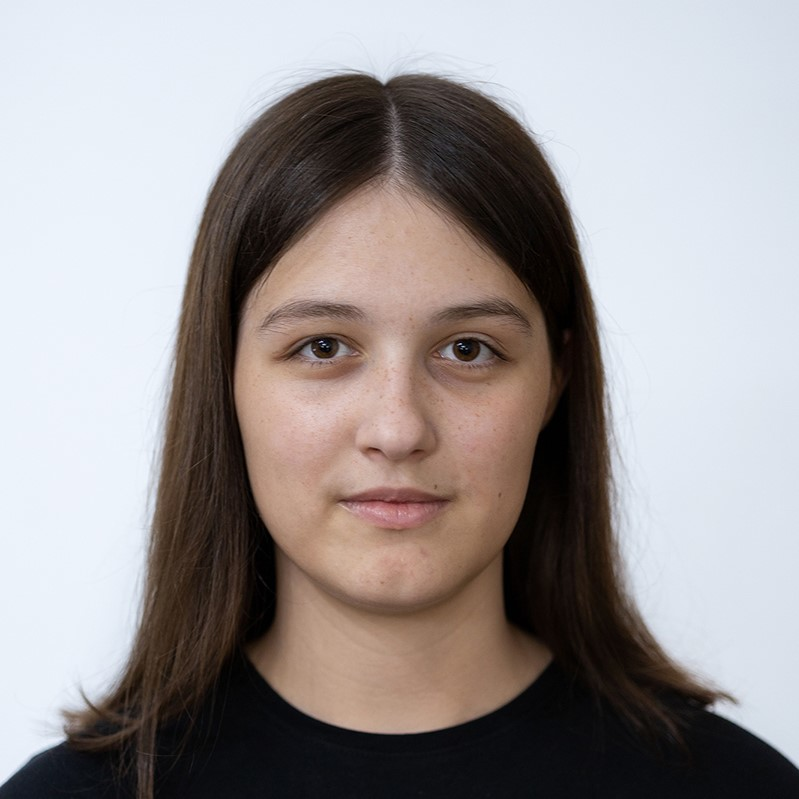
\includegraphics[width=3.5cm]{res/cover/A104437.png} &
            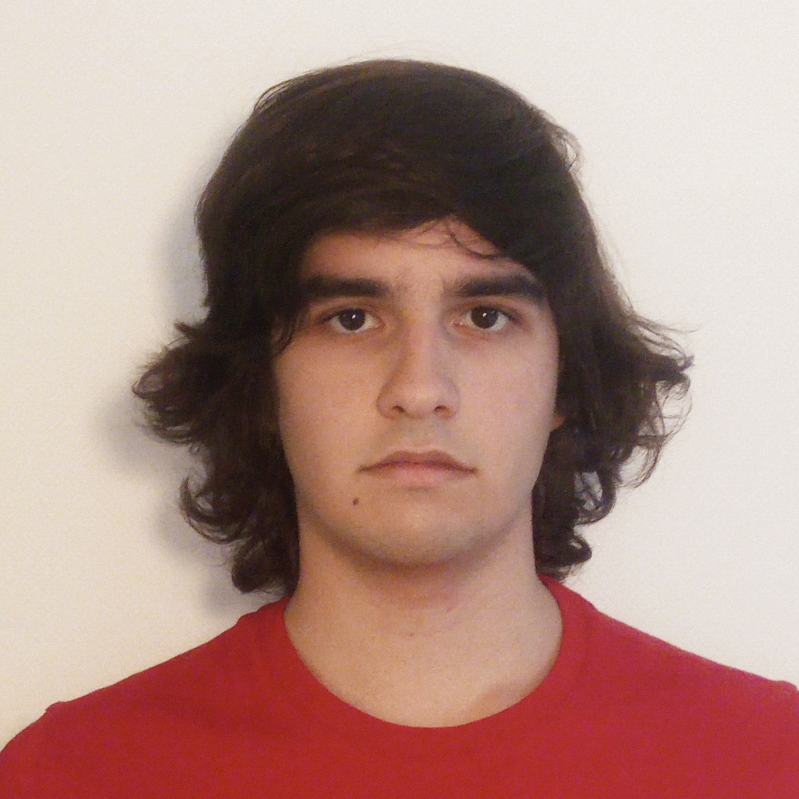
\includegraphics[width=3.5cm]{res/cover/A104348.png} &
            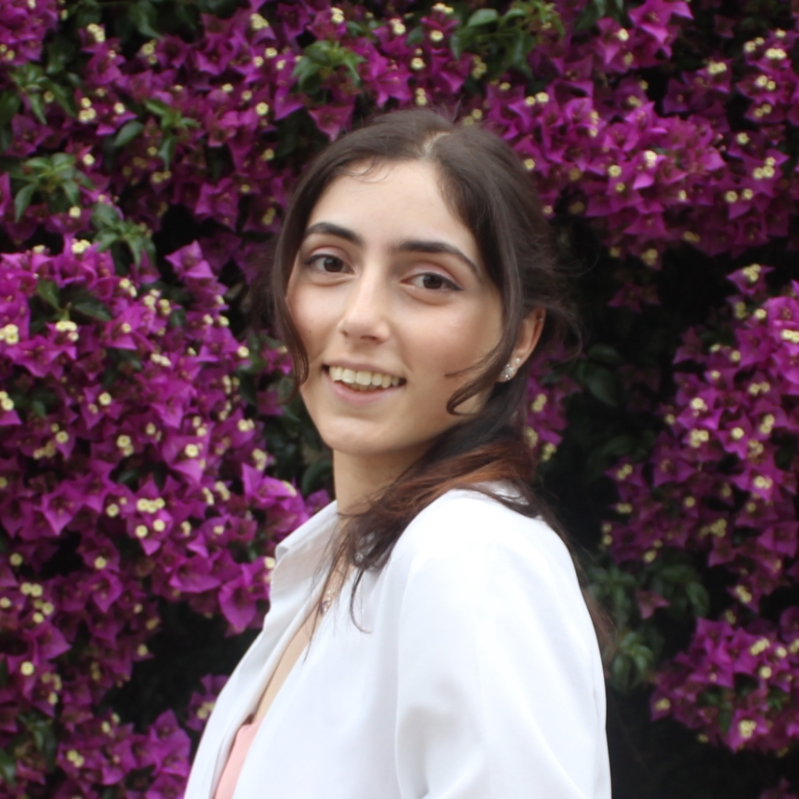
\includegraphics[width=3.5cm]{res/cover/A90817.png} &
            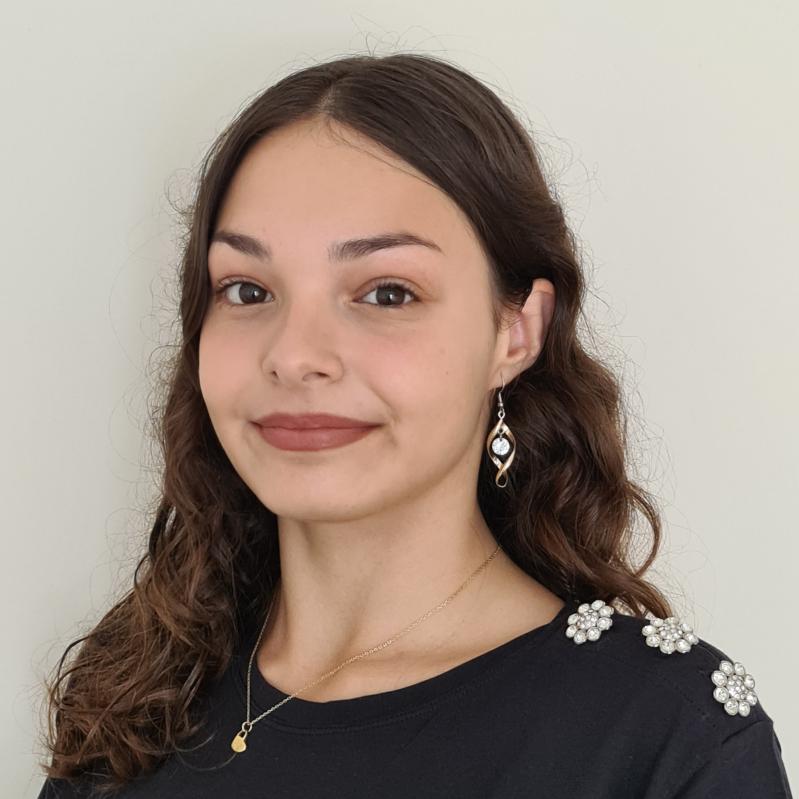
\includegraphics[width=3.5cm]{res/cover/A104179.png} \\

            Ana Oliveira & Humberto Gomes & Mariana Cristino & Sara Lopes \\
            A104437      & A104348        & A90817           & A104179
        \end{tabular}
    \end{center}
\end{adjustwidth}

\pagebreak

\begin{abstract}
    \textbf{\color{red} TODO - resumo}
\end{abstract}

\section{Transformações}

\textbf{\color{red} TODO - transformações}

\section{Modelo estático do sistema solar}

\textbf{\color{red} TODO - sistema solar}

\section{Extras}

\subsection{UI (Interface Gráfica)}

A interface do projeto foi desenvolvida com o auxílio da biblioteca \texttt{ImGui}. Esta biblioteca
simplifica a gestão e atualização dos componentes, pois os elementos gráficos são recriados a cada
\textit{frame}.

A classe responsável pela configuração e renderização da interface é a \texttt{UI}.
Assim, no processo de inicialização realizado no construtor da classe, a criação do contexto
\texttt{ImGui} é realizada (garante que a biblioteca encontra-se bem configurada), bem como a
configuração do estilo da interface (aqui, o estilo \textit{Dark} foi escolhido para se obter uma
melhor visualização dos elementos gráficos) e é efetuada a inicialização das implementações para a
\texttt{OpenGL} e \texttt{GLFW} (assegura que há compatibilidade entre o motor de renderização
utilizado com o sistema de janelas).

A interface é composta por um menu principal, sendo este renderizado na função \texttt{UI::render
(int renderedEntities)} com as seguintes opções:

\begin{itemize}
    \item Acompanhamento do Desempenho:
    \begin{itemize}
        \item FPS (\textit{Frames Per Second}): apresenta o número de \textit{frames}
        renderizados por segundo.
        \item Apresenta o número de entidades renderizadas em relação ao número total de entidades
        existentes.
    \end{itemize}
    \item Configurações:
    \begin{itemize}
        \item Preenchimento de polígonos: permite alternar entre o preenchimento
        (\textit{fill polygons}) e o modo \textit{wireframe}.
        \item \textit{Back face culling}: ativa ou desativa o \textit{back-face culling}.
        \item Exibir eixos: ativa ou desativa a visualização dos eixos.
        \item \textit{Bounding spheres}: ativa ou desativa a visualização das esferas delimitadoras
        das entidades.
    \end{itemize}
    \item Câmara: permite modificar as coordenadas da posição da câmara.
\end{itemize}

Após a definição dos elementos gráficos, a interface é renderizada através da função
\texttt{ImGui::Render()} e pelo \texttt{ImGui\_ImplOpenGL3\_RenderDrawData(ImGui::GetDrawData())}.

\begin{figure}[H]
    \centering
    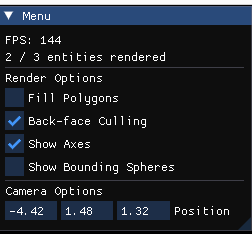
\includegraphics[width=0.35\textwidth]{res/phase2/UI.png}
    \caption{Interface Gráfica.}
\end{figure}

\section{Resultados obtidos}

\textbf{\color{red} TODO - resultados}

\section{Conclusão e Trabalho Futuro}

\textbf{\color{red} TODO - conclusão}

\begingroup
\section{Bibliografia}
\renewcommand{\section}[2]{}

\begin{thebibliography}{9}
    \bibitem{exemplo}
        \href{https://youtu.be/dQw4w9WgXcQ}{Um item de exemplo na bibliografia}
\end{thebibliography}
\endgroup

\end{document}
